\documentclass[11pt]{article}
\usepackage[margin=0.85in]{geometry}
\usepackage{graphicx}
\usepackage{amsmath}
\usepackage[colorlinks=true,urlcolor=blue]{hyperref}

\title{Extracting 1D Spectra from JADES NIRSpec Images}
\author{}
\date{}

\begin{document}
\maketitle
\vspace{-2em}
\noindent
I used Python to extract 1D spectra from 3,752 calibrated 2D JADES NIRSpec
CLEAR/PRISM spectra and compared them with the corresponding published 1D data.
The code and example plots are in the
\href{https://colab.research.google.com/drive/1-L3NN1DscB1QbgjsxSdwaJ_2WfMDQp-y}{Google Colab notebook}.

\section*{Method}
I read the 2D flux image and wavelength grid from each FITS file with Astropy.
Each column is a wavelength bin, and each row is a position along the slit.
The line \verb|np.nansum(image, axis=0)| adds the spatial rows to give one flux
value per wavelength. I marked columns with only NaN values as missing.
Before plotting, I checked that the extracted and published spectra used the
same wavelength grid.

\section*{Results}
The full-row sum differs from the published spectrum because it includes
pixels outside the source trace. In Figure 1, the bright band near the middle
shows the source. The blue bands above and below it have negative flux left
by background subtraction. Adding these pixels lowers the total flux at
some wavelengths.

\begin{center}
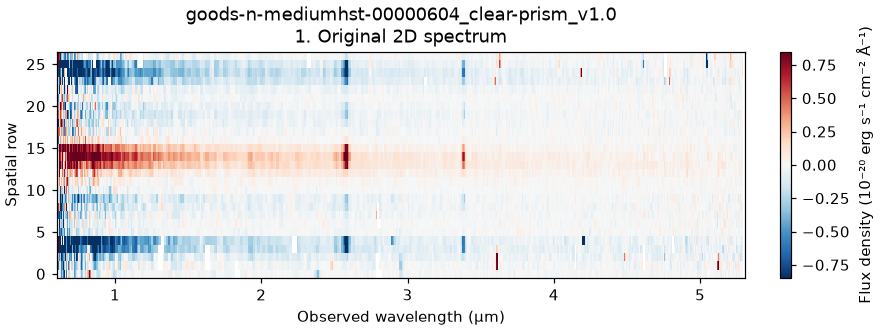
\includegraphics[width=0.82\linewidth]{stage1.png}\par
\small Figure 1. The 2D spectrum of GOODS-N target 604. The red strip near the middle shows
the source, and the blue strips show negative flux.

\end{center}

\clearpage
\section*{1D comparison for GOODS-N target 604}

\begin{center}
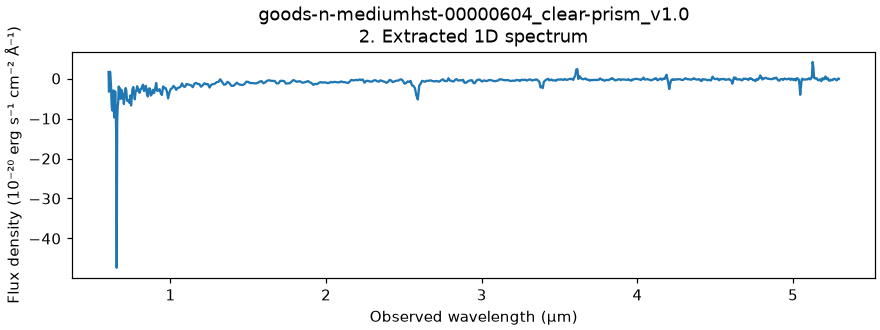
\includegraphics[width=0.82\linewidth]{stage2.png}\par
\small Figure 2. The 1D spectrum obtained by adding all spatial rows.

\medskip
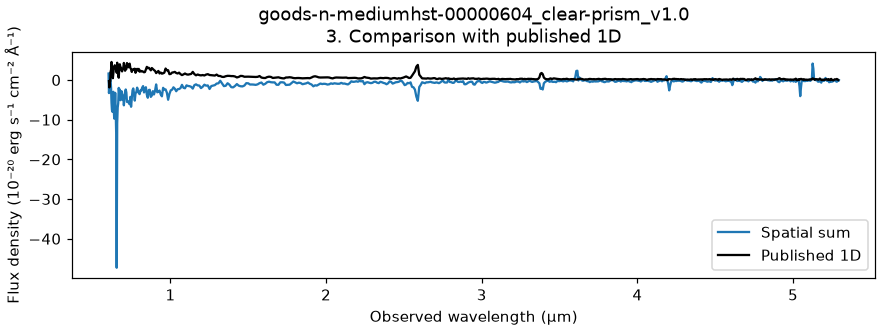
\includegraphics[width=0.82\linewidth]{stage3.png}\par
\small Figure 3. The full-row sum in blue and the published spectrum in black.
The difference is easiest to see at short wavelengths.
\end{center}

\noindent
JADES uses a five-pixel region around the source. To see what difference
the number of rows made, I tried summing only the middle five rows for the
first 15 spectra. This gave a closer match for all 15. I measured the difference
using the root-mean-square error (RMSE) between the two curves. The median
RMSE fell by about a factor of nine. The five-row sum better matches the spatial aperture used by JADES.

\end{document}
